\documentclass[12pt]{article}

\usepackage{wrapfig}
\usepackage[spanish]{babel}
\usepackage[utf8]{inputenc}
\usepackage{amsmath}
\usepackage{graphicx}
\usepackage[colorinlistoftodos]{todonotes}

\begin{document}

\begin{titlepage}

\newcommand{\HRule}{\rule{\linewidth}{0.5mm}} % Defines a new command for the horizontal lines, change thickness here

\center % Center everything on the page
 
%----------------------------------------------------------------------------------------
%	HEADING SECTIONS
%----------------------------------------------------------------------------------------

\textsc{\LARGE Universidad de Sonora} \\ [0.4cm]

\includegraphics[scale=.65]{./Images/Logo} \\ [0.3cm]
\textsc{\LARGE Física computacional I}\\[0.3cm]

%----------------------------------------------------------------------------------------
%	TITLE SECTION
%----------------------------------------------------------------------------------------

\HRule \\

{\huge \bfseries
Actividad 2\\
Iniciando el análisis de datos\\
con la biblioteca Pandas de\\
Python\\}

 \HRule \\[1cm]

%----------------------------------------------------------------------------------------
%	DATE SECTION
%----------------------------------------------------------------------------------------

\vfill

\begin{minipage}{0.6\textwidth}
%\begin{flushleft}
	\raggedright
	{\large \textbf{Gómez García, Manuel Ignacio}}
%\end{flushleft}
\end{minipage}
~
\begin{minipage}{0.35\textwidth}
%\begin{flushright}
	\raggedleft
	{\large \textbf{8/Diciembre/2018}}
%\end{flushright}
\end{minipage}

\end{titlepage}

\section{Introducción}

\noindent En la presente práctica de Python, hicimos uso de un cuadernillo de trabajo generado en Jupyter notebook y trabajamos con las bibliotecas de Panda y Matplotlib para analizar los datos recabados por las Estaciones Meteorológicas Automáticas (EMAS)\footnote{http://smn.cna.gob.mx/es/estaciones-meteorologicas-automaticas-2} del Servicio Meteorológico Nacional de CONAGUA. \\
\indent Hay que tener en cuenta que el objetivo principal de esta actividad consiste en aprender a manejar series de datos haciendo uso de Pandas para finalizar creando dos gráficos distintos y poder analizar los datos tras esto.

\section{Desarrollo del código}

\noindent A continuación veremos paso a paso cómo fue que se manejaron los datos y posteriormente, la creación de las gráficas con los mismos.

\subsection{Importación de bibliotecas y datos}

\noindent En el bloque de código [1] podemos ver que importamos las bibliotecas necesarias y además, hacemos uso del comando mágico \textbf{\%matplotlib inline} para que los gráficos que creemos se muestren dentro del cuadernillo; el bloque [2] muestra la configuración utilizada para leer el archivo .CSV 	que contiene las lecturas de la estación.

\begin{figure}[h!]
	\center
	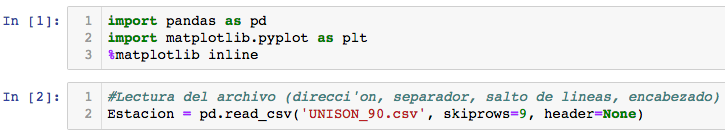
\includegraphics[scale=.6]{./Images/importacion}
	\caption{\label{fig:importacion} Importando bibliotecas y leyendo el archivo .CSV.}
\end{figure}

\pagebreak

\subsection{Reordenando datos y formatos}

\noindent Lo siguiente a tratar son los encabezados de cada columna pues no cuentan con un nombre, así que habremos de asignárselos nosotros mismos.

\begin{figure}[h!]
	\center
	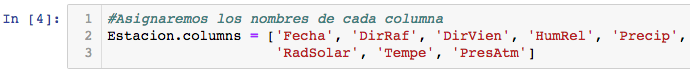
\includegraphics[scale=.6]{./Images/columnas}
	\caption{\label{fig:columnas} Cada columna es nombra apropiadamente.}
\end{figure}

\noindent Al verificar los tipos de cada elemento en el marco de datos podremos ver que la columna \textbf{Fecha} es simplemente marcada como un objeto cuando debería ser reconocido como \textbf{datetime}, así que modificaremos eso en el bloque [7].

\begin{figure}[h!]
	\center
	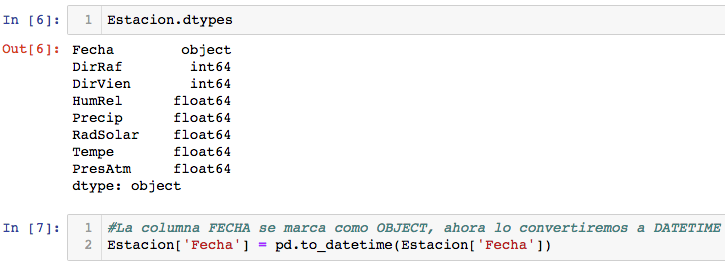
\includegraphics[scale=.6]{./Images/tipo}
	\caption{\label{fig:tipo} Modificamos el tipo de la columna \textbf{Fecha}.}
\end{figure}

\subsection{Nuevo marco de datos}

\noindent Nuestro próximo paso consiste en obtener un nuevo marco de datos que contenga la información de 10 días, los cuales nosotros podremos elegir al momento de introducir la fecha en la condición lógica para delimitar la selección del bloque [10] (Véase la figura \ref{fig:dias}).

\begin{figure}[h!]
	\center
	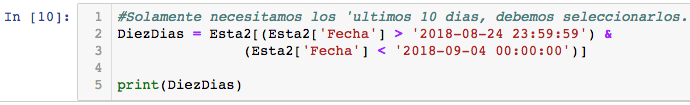
\includegraphics[scale=.6]{./Images/dias}
	\caption{\label{fig:dias} Delimitamos la selección con una condición lógica.}
\end{figure}

\subsection{Gráficos}

\noindent En este punto tenemos bien ordenados los datos y simplemente resta configurar cada una de las gráficas a crear. \\
\indent La primer gráfica es generada con el código del bloque [11].

\begin{figure}[h!]
	\center
	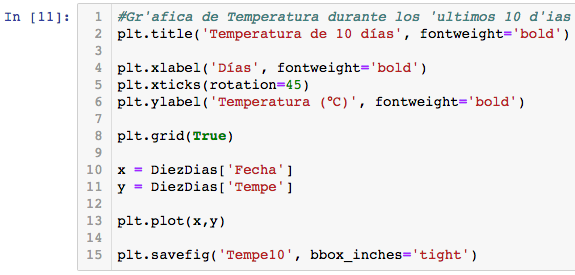
\includegraphics[scale=.6]{./Images/config1}
	\caption{\label{fig:config1} Configuración de la gráfica de temperatura.}
\end{figure}

Con los comandos mostrados podemos genera una gráfica igual a la que veremos en la figura \ref{fig:tempe}.

\begin{figure}[h!]
	\center
	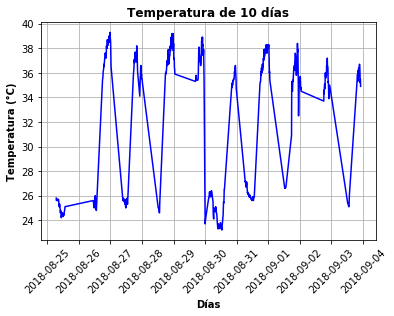
\includegraphics[scale=.6]{Tempe10}
	\caption{\label{fig:tempe} Temperatura contra tiempo durante 10 días.}
\end{figure}

Los comandos para generar la segunda gráfica se muestran en la figura \ref{fig:config2}, la cual corresponde al bloque de código [12], el mismo que permite generar una gráfica que podemos apreciar en la figura \ref{fig:pres}.

\begin{figure}[h!]
	\center
	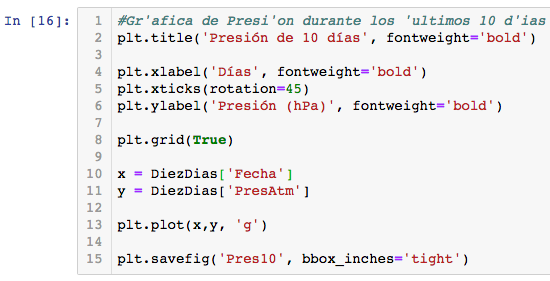
\includegraphics[scale=.58]{./Images/config2}
	\caption{\label{fig:config2} Configuración de la gráfica de presión.}
\end{figure}

\begin{figure}[h!]
	\center
	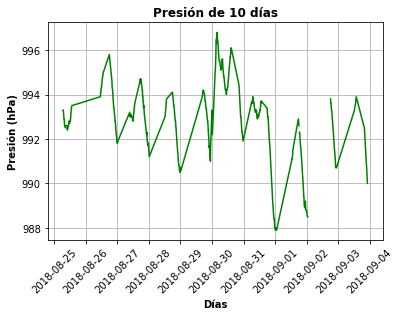
\includegraphics[scale=.6]{Pres10}
	\caption{\label{fig:pres} Presión contra tiempo durante 10 días.}
\end{figure}

\section{Conclusión}

Tras llevar a cabo este código podemos ver lo útil que resulta la biblioteca de Pandas a la hora de manejar marcos de datos pues cuentan con una amplia lista de comandos con los cuales podemos resolver y aplicar un tratamiento de "limpieza" a los conjuntos de información que obtengamos. \\
\indent Si bien queremos dar una opinión acerca de lo visto en las gráficas, podemos mencionar que parecen estar inversamente relacionados los datos analizados pues cuando el valor de la presión disminuye la temperatura sufre un incremento.

\section{Apéndice}
\begin{enumerate}
\item \textbf{¿Cuál es tu impresión de trabajar con Python en Jupyter?} \\ [0.15cm]
Parece hacer todo mucho más sencillo por la gran cantidad de ventajas que ofrece, además de hacer un poco más visual todo, es bastante amigable con el usuario.

\item \textbf{¿Cuál es tu primera impresión de trabajar con Pandas?} \\ [0.15cm]
La biblioteca de Pandas cuenta con una gran cantidad de funciones muy útiles cuando se trata de manejar los marcos de datos, parece ser más que suficiente por el momento.

\item \textbf{¿Qué partes se te dificultaron más?} \\ [0.15cm]
Lo más complicado siento que fue aplicarle un "tratamiento" a los datos para que fuera más sencillo trabajarlos, en la forma y formato adecuado.

\item \textbf{¿Qué te pareció esta Actividad? ¿Alcanzó el tiempo?} \\ [0.15cm]
Creo que la actividad es bastante apropiada para dar una introducción al análisis de datos pues la biblioteca de Pandas veo que cuenta con un gran respaldo por parte de muchos usuarios, haciéndola un elemento indispensable para este tema. 

\item \textbf{¿Qué le agregarías o quitarías a esta actividad?} \\ [0.15cm]
Me gustaría que la actividad tuviera otra cosa más por hacer, así como una gráfica doble para apreciar mejor el comportamiento de los datos.

\item \textbf{¿Qué cosas te parecieron interesantes y qué se te hizo aburrido?} \\ [0.15cm]
Lo interesante sería el comenzar a manejar un nuevo lenguaje y utilizar Jupyter Notebook; lo aburrido, podría decirse que es al momento de buscar información para realizar lo que se desea pues en ocasiones se visita una página que no ofrece buena información, ejemplos o aquello que buscamos.

\end{enumerate}

\begin{thebibliography}{1}
	\bibitem{EMAS} Mapa de Estaciones Meteorológicas Automáticas (EMAS)(versión 2014-2017). Recuperado de http://smn.cna.gob.mx/es/estaciones-meteorologicas-automaticas-2
	
\end{thebibliography}

\end{document}